\documentclass[11pt,a4paper]{article}

%  PREÁMBULO -

\usepackage[utf8]{inputenc}
\usepackage[pdftex]{graphicx}
\usepackage[spanish,es-tabla]{babel}
\usepackage{amsmath}
\usepackage{amsfonts}
\usepackage{url}
\usepackage{cprotect}
\usepackage{siunitx}
\usepackage{longtable,tabularx}
\usepackage{lastpage}
\usepackage[colorlinks=true,linkcolor=black,urlcolor=blue]{hyperref}
\usepackage{apacite}
\usepackage{afterpage}
\usepackage[table,xcdraw]{xcolor}
\usepackage{lscape}
\usepackage{multirow}
\usepackage{longtable}
\usepackage{pdfpages} %Agregar un PDF externo al documento
\usepackage{cancel}
\usepackage{tcolorbox}
\tcbuselibrary{theorems}
\usepackage{txfonts}
\usepackage[left=2cm,right=1.5cm,top=3cm,head=2cm,bottom=2cm]{geometry}
\usepackage{lastpage}
\usepackage{fancyhdr}
\usepackage{titlesec}
\usepackage[export]{adjustbox}
\pagestyle{fancy}

\titleformat{\subsubsection}
  {\normalfont\normalsize\bfseries}
  {\hspace{2em}\thesubsubsection} % <- número con sangría
  {1em}                            % <- espacio entre número y título
  {}                               % <- antes del texto del título
%--------------------------------------------------------------------------------------------------------------------------
%  INICIO DEL DOCUMENTO - FORMATO UNC - FCEFyN
%--------------------------------------------------------------------------------------------------------------------------

\begin{document}

\begin{titlepage}

\noindent
\begin{minipage}[c]{0.2\textwidth}
  
\includegraphics[width=\linewidth]{Logo-fcenuba.png}
\end{minipage}
\hfill
\begin{minipage}[c]{0.4\textwidth}
  \centering
  \vspace*{5.5em}  % opcional: para bajar el texto si queda muy arriba
  {UNIVERSIDAD DE BUENOS AIRES \par}
  \vspace{0.1cm}
  {\large Facultad de Ciencias Exactas y Naturales\par}
  \vspace{0.1cm}
  {\large Departamento de Ciencias Geológicas \par}
\end{minipage}
\hfill
\begin{minipage}[c]{0.2\textwidth}
  
\includegraphics[width=\linewidth]{Logo_Geologia.png}
\end{minipage}

% \noindent
% {
\includegraphics[width=0.2\textwidth]{Logo-fcenuba.png} }

% \noindent
% \hfill
% {
\includegraphics[width=0.2\textwidth]{Logo_Geologia.png}\par}


\centering

% \vspace{0.5cm}

% \vspace{0.2cm}
% {\Large Facultad de Ciencias Exactas y Naturales \par}
% \vspace{0.2cm}
% {\Large Departamento de Ciencias Geológicas \par}
\vspace{2cm}
{\huge Geología de las nacientes del río Malargüe, provincia de Mendoza \par} %título del TFL
%\vspace{3cm}
%{\itshape\Large Resumen \par}
\begin{figure}[h]
    \centering
    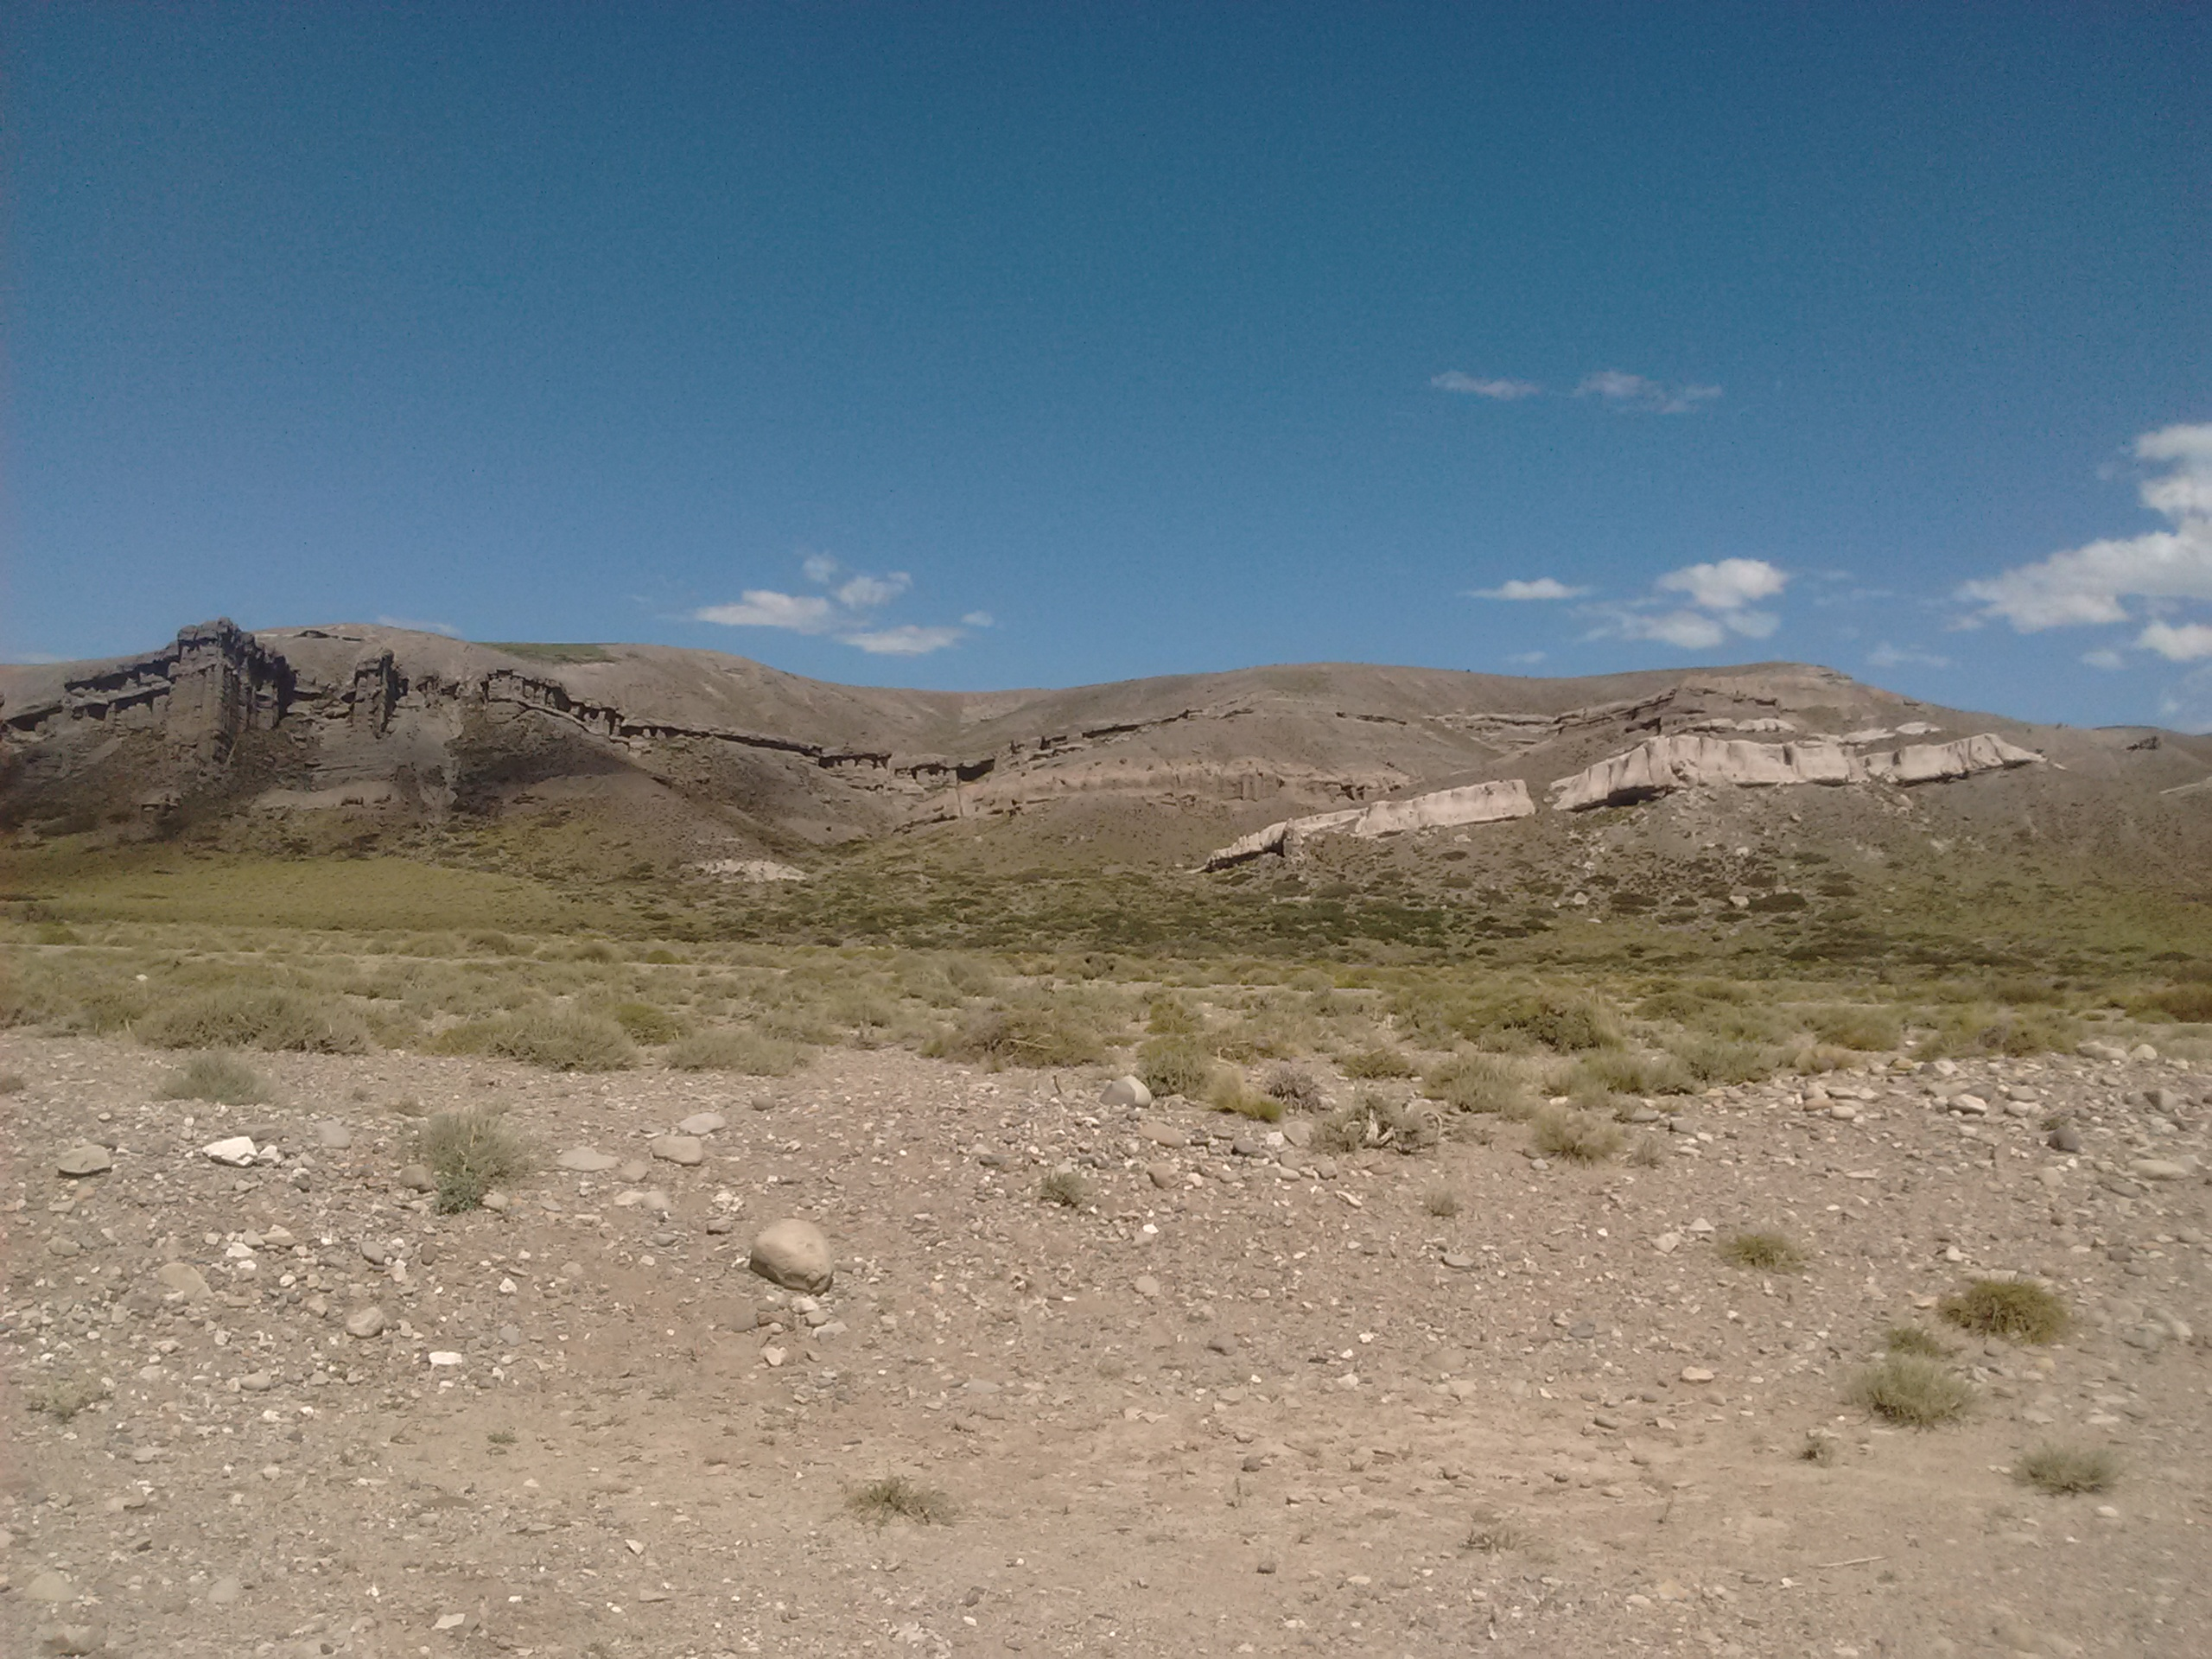
\includegraphics[width=.7\linewidth]{IMG_20160223_152527650.jpg}
    %\caption{}
    \label{fig:enter-label}
\end{figure}
\vfill
{\Large Autor: \par}
{\Large \textbf{\emph{Ricardo Tapia}} \par}%nombre autor/autora
\vspace{0.5cm}
{\Large Director/a: \par}
{\Large \textbf{\emph{Dr. Bruno Díaz}} \par}%nombre director/directora
\vfill
{\Large Abril 2025 \par}
\end{titlepage}

\fancyhead{}
\fancyhf{}
\fancyfoot{}
\newpage

%-----------------------------------------------------------------------------------------------------------------------------------------------------------Resumen
%-----------------------------------------------------------------------------------------------------------------------------------------------------------
\thispagestyle{empty}
\section*{\Huge Resumen}
El Trabajo de Licenciatura (TFL) es obligatorio, autónomo bajo la supervisión de uno o dos directores. El objetivo del mismo es  consolidar e integrar los conocimientos teórico-prácticos. Demostrar la capacidad para programar y realizar un trabajo geológico de investigación básica o aplicada y/o profesional.\par
El TFL estará organizado en forma coherente y clara y debe incluir obligatoriamente mapas y perfiles geológicos. Deberá estar escrito a computadora, a espacio y medio, en papel blanco, liso, tamaño A4.\par
La carátula deberá incluir en su parte superior “Universidad de Buenos Aires, Facultad de Ciencias Exactas y Naturales, Departamento de Ciencias Geológicas”, a continuación, el título del trabajo (que incluya ubicación geográfica), nombre del autor/a, Director/a, Codirector/a y año.\par
El texto deberá constar de un Índice de capítulos y subcapítulos. También incluirá una página de agradecimientos donde conste las personas que han colaborado en tareas específicas del TFL.\par
La información reunida se estructurará aprox. de la siguiente manera:
\begin{itemize}
    \item Breve resumen del tema considerado y objetivos.
    \item Introducción en la que consignará la metodología utilizada, la ubicación de la zona de estudio, antecedentes, etc.
    \item Descripción geológica general del área.
    \item Descripción detallada de las unidades estudiadas, su estructura, geomorfología, análisis sedimentario, etc.
    \item En un ítem independiente se realizará la interpretación de todo el material analizado y desarrollado en capítulos previos.
    \item En un capítulo final se explicarán las conclusiones a las que se ha llegado.
    \item Referencias bibliográficas.
\end{itemize}

 Las ilustraciones y fotografías deberán estar acompañadas por una explicación detallada del concepto o dato geológico que pretenden ilustrar. Deberán estar mencionadas en el texto.\par
 En todas las descripciones de muestras, cortes, pulidos, fósiles, etc. incluidos en el texto, deberá hacerse referencia específica al número de muestra correspondiente, ya sea entre paréntesis o como parte del discurso, en forma lo suficientemente clara como para que un posible revisor de dichos elementos pueda verificar lo expresado en el texto. Se recomienda especialmente la precisa localización de esta información en los mapas y perfiles. \par
 En caso de utilizar fuentes preexistentes para la realización de mapas, éstas deberán ser adecuadamente reconocidas (citadas).\par
 Este archivo es un resumen y sirve de guía para la confección de TFL. Es una sugerencia y puede ser modificado dentro de las normas establecidas para la confección del TFL.\par
 Este archivo fue confeccionado en \LaTeX{} y el código para hacer el TFL en este sistema de composición de texto está disponible en \textsf{Overleaf} en la sección de \textit{templat}e con el nombre  \textbf{\textit{Tesis Licenciatura Geología FCEN-UBA }}








\newpage
%-----------------------------------------------------------------------------------------------------------------------------------------------------------Agradecimientos
%-----------------------------------------------------------------------------------------------------------------------------------------------------------
\thispagestyle{empty}
\section*{\Huge Agradecimientos}
Se agradace a todas las personas que participaron en la confección de este documento y del código de \LaTeX{}.
\newpage
%-----------------------------------------------------------------------------------------------------------------------------------------------------------Indice de contenidos
%---------------------------------------------------------------------------------------------------------------------------------------------------------
\thispagestyle{empty}
\renewcommand\contentsname{\textbf{\Huge Índice}}
    \begin{center}
       \tableofcontents
       
    \end{center}
    
\clearpage           
\addtocontents{toc}{~\hfill\textbf{Página}\par}  



%------------------------------------------------------------------------------------------------------------------------------------------------Configuración de los encabezados y pié de página
%--------------------------------------------------------------------------------------------------------------------------
\newpage
\fancyhead{}
\fancyhf{}
\fancyhead[L]{\textit{\nouppercase\textbf{\leftmark}}} %Nombre de la sección en el encabezado
\renewcommand{\sectionmark}[1]{\markboth{#1}{}} %quita el numero de sección en el encabezado.
\fancyhead[R]{\emph{Ricardo Tapia}} %nombre del autor en el encabezado
%
\includegraphics[width=0.05\textwidth]{Logo-fcenuba.png} 

\renewcommand{\headrulewidth}{2pt} 
\renewcommand{\footrulewidth}{1pt}

%\lfoot{
\includegraphics[width=0.1\textwidth]{Logo_Geologia.png}} % imagén en el pie de página
\rfoot{\thepage \; de \;\pageref{LastPage}}

%-----------------------------------------------------------------------------------------------------------------------------------------------------------Introducción
%-----------------------------------------------------------------------------------------------------------------------------------------------------------

\setcounter{figure}{0} %reincia la numeración de las figuras
\renewcommand{\thefigure}{\thesection.\arabic{figure}}
\section{\Large Introducción}

\subsection{\large Motivación/Problemática del estudio}

       Indicar contexto de la tesis. Deben mencionarse las palabras claves, de lo que trata la tesis.\par
  
       Indicar antecedentes que guarden relación con la problemática de la tesis. Un contexto más específico.\par
       

       Si no quedó planteado en el párrafo anterior, en este párrafo debe plantearse la problemática. Usualmente va seguida de una conjunción tal como: Sin embargo, a pesar de esto, no obstante. A veces, algunos autores manifiestan la problemática de manera más explícita poniéndola como una pregunta entre signos de interrogación.\par
 
       Antecedentes específicos acerca de cómo otros autores han aportado en la resolución de dicho problema. Este párrafo también debe dar luces de la hipótesis del trabajo.\par

       Indicar cómo se abordará el problema; es decir, qué metodologías utilizará, qué datos nuevos presentará y qué tipo de análisis hará con ellos.

           
    \begin{figure}[h]
        \centering
        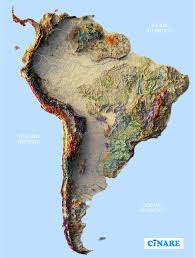
\includegraphics[width=0.3\linewidth]{images1.jpg}
        \caption{Mapa geológico regional de Sudamérica}
        \label{fig:mapareg}
    \end{figure}
            
\subsection{\large Hipótesis y Objetivos}
    
       En la hipótesis se debe indicar el modelo o posible solución al problema planteado y de qué manera los resultados que espera sostienen dicho modelo o solución. \par
     
       Se puede separar en Objetivo General o Principal y específicos o secundarios. \par
   
        En el objetivo principal se plantea de manera explícita que, a través de los resultados de este trabajo, se pretende resolver el problema planteado en la introducción o fortalecer un modelo que lo explique.\par
         
        En los objetivos específicos se debe indicar las etapas que deben cumplirse para lograr el objetivo general. Debe responder a la pregunta: \textbf{¿Para qué realizaré cada parte del trabajo?} Cada uno de los objetivos específicos debe apuntar a la resolución del objetivo general. Si no es así, significa que el objetivo específico no corresponde o que el objetivo general quedo mal planteado.

        
        \subsection{\large Metodologías}
Indicar los métodos que utilizará para llevar a cabo cada uno de los objetivos específicos que deben cumplirse para lograr el objetivo general. Debe responder a la pregunta: \textbf{¿Cómo realizaré cada parte del trabajo?} Cada una de las metodologías debe apuntar a la resolución de un objetivo específico. Si no es así, significa que la metodología no corresponde. A su vez, debe existir a lo menos una metodología que permita resolver cada objetivo específico, de lo contrario, la metodología no estaría completa.\par
            deberá escribirse la explicación detallada de los procedimientos seguidos e instrumental usado en las tareas de campo, laboratorio y gabinete.
     
        \subsection{\large Características del área de estudio}
            \subsubsection{Ubicación y acceso}
            Indicar vías de acceso y tipo de movilización que se requiere para acceder al área de estudio.
            \begin{figure} [h] %[h] fuerza a que la fig. se ubique en este lugar.
                \centering
                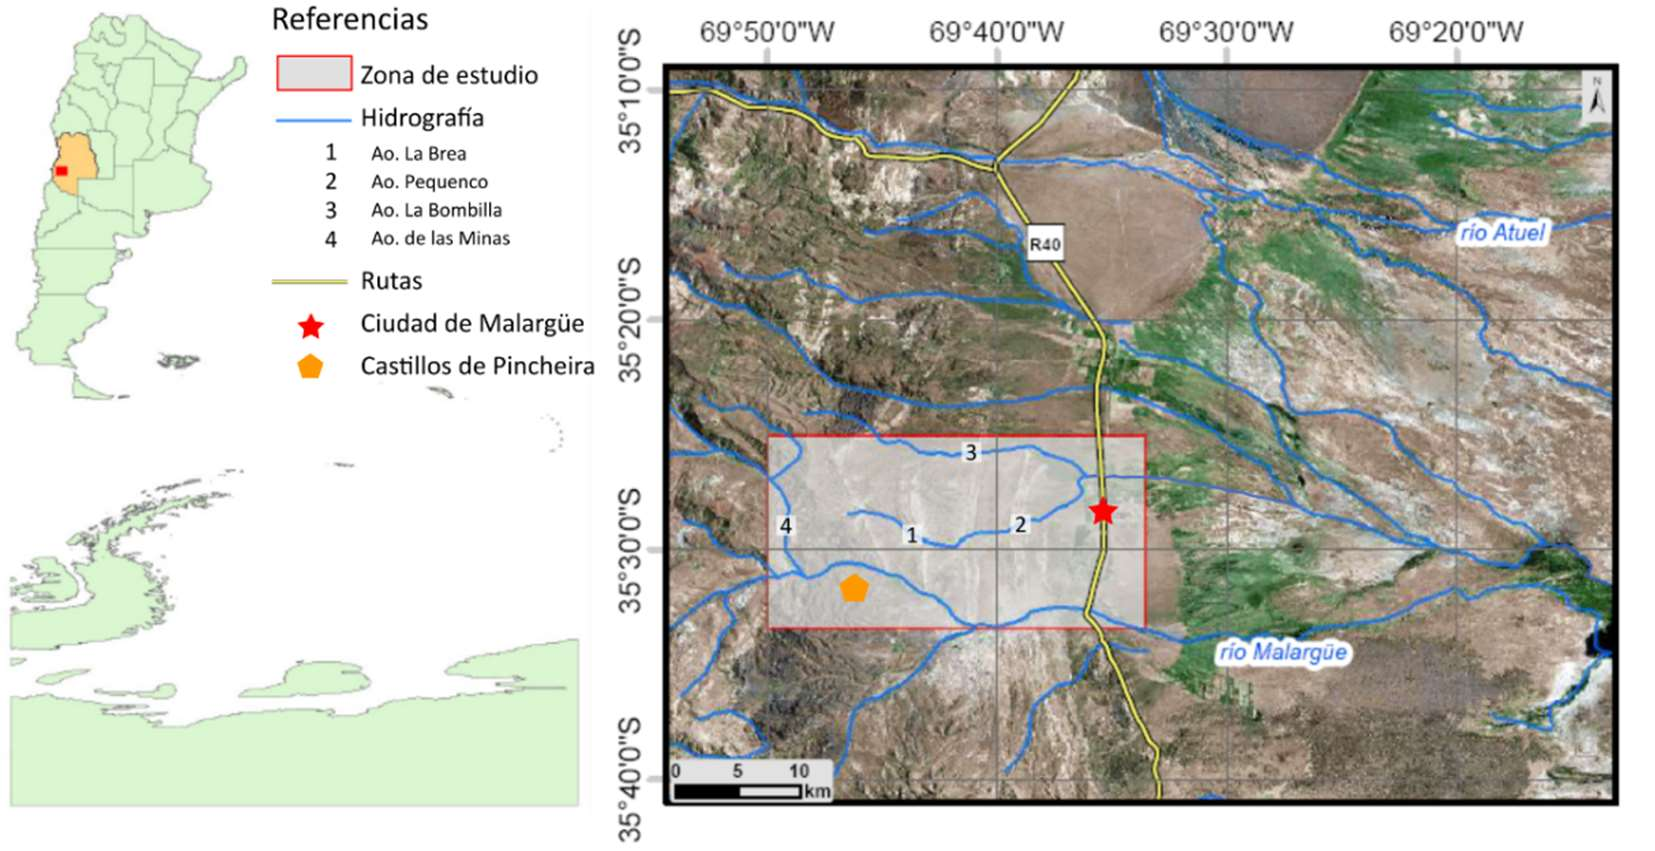
\includegraphics[width=0.7\linewidth]{Fig. ubicacion.jpg}
                \caption{\small Mapa de ubicación de la zona de estudio. En la imagen satelital de la derecha se marca con un rectangulo rojo el área de estudio.}
                \label{fig:enter-label}
            \end{figure}
            \subsubsection{Geografía}
             Se puede o no agregar esta subsección. Si se la considera entonces se deben agregar algunas características relevantes de la zona y que sean necesarias mencionar en el contexto de la tesis. 
            \subsubsection{Clima}
             Se puede o no agregar esta subsección. Si se la considera entonces se deben agregar algunas características relevantes de la zona y que sean necesarias mencionar en el contexto de la tesis. 
            \subsubsection{Hidrología}
            Se puede o no agregar esta subsección. Si se la considera entonces se deben agregar algunas características relevantes de la zona y que sean necesarias mencionar en el contexto de la tesis. 
            \subsubsection{Flora y Fauna}
            Se puede o no agregar esta subsección. Si se la considera entonces se deben agregar algunas características relevantes de la zona y que sean necesarias mencionar en el contexto de la tesis. 
        \subsection{\large Antecedentes}
            Se deben mencionar los principales trabajos previos que se realizaron en el área de estudio y los principales aportes de cada uno de ellos al conocimiento geológico del área de estudio. Hacer énfasis en los trabajos que abordaron temáticas o resultados que tienen que ver con la problemática de la tesis.

\newpage          

%-----------------------------------------------------------------------------------------------------------------------------------------------------------Marco Geológico
%-----------------------------------------------------------------------------------------------------------------------------------------------------------
\setcounter{figure}{0} %reincia la numeración de las figuras
\renewcommand{\thefigure}{\thesection.\arabic{figure}}
\section{\Large Marco Geológico}
Debe dar referencia a los aspectos geológicos que serán citados en este trabajo. Puede o no ir separado en ítems como a continuación.
        \subsection{\large Marco Tectónico/Geodinámico}
        En esta subsección se puede hablar del marco tectónico actual en la que se enmarca el área de estudios tal como tipo de margen tectónico, placas tectónicas, velocidades de las placas, etc.

        \begin{figure} [h]
            \centering
            \includegraphics[width=0.4\linewidth]{fig. margo tectónico.jpg}
            \caption{\small a) Configuración tectónica desde el Cretácico hasta la actualidad (modificada de Zonenshayn et al., 1984). b) Compilación de la tasa de convergencia promedio y la oblicuidad promedio entre las placas de Nazca (Farallón) y Sudamericana. En verde Pardo-Casas y Molnar (1987) y en negro Somoza (1998). c) Reconstrucción del moviendo de dos puntos de la Placa de Nazca a partir del Cretácico (Pardo-Casas y Molnar, 1987).}
            \label{fig:enter-label}
        \end{figure}
              
        También se pueden mencionar y describir las principales provincias geológicas o unidades morfoestructurales que se disponen en un contexto regional que contenga al área de estudio.

        
        \begin{figure} [h]
            \centering
            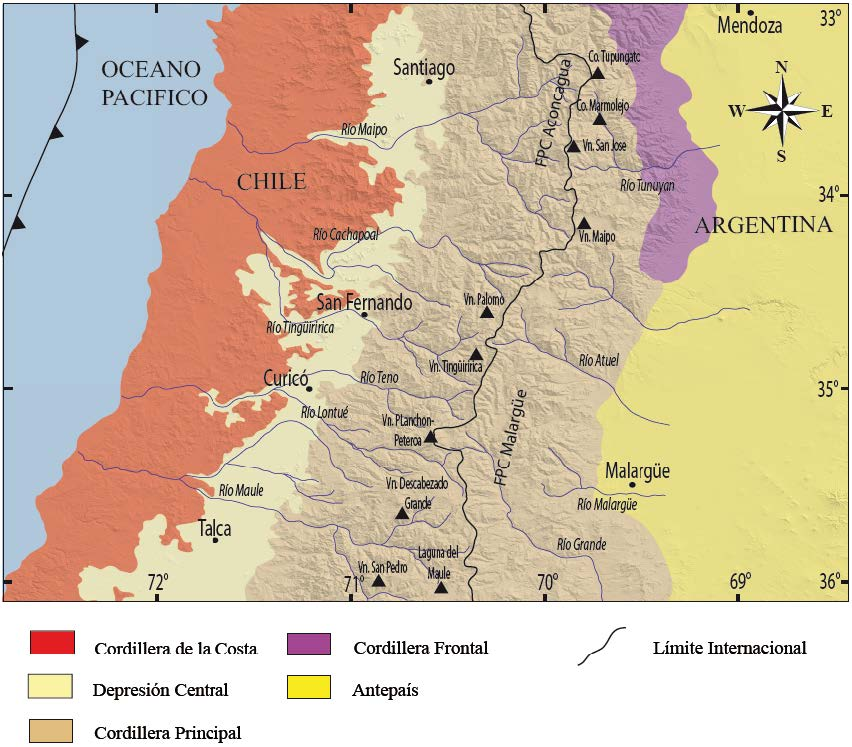
\includegraphics[width=0.5\linewidth]{Fig. provincias.jpg}
            \caption{\small Principales morfoestructuras o provincias geológicas entre los 33°S y 36°S.}
            \label{fig:enter-label}
        \end{figure}
       
        
        En esta subsección se puede hablar de la historia o evolución geológica más regional que enmarca al área de estudio. Si luego se decide escribir un capítulo de geología del área de estudio donde se describan las unidades estratigráficas del área en cuestión, entonces se sugiere evitar hacer una descripción de esas unidades en este apartado para que no se repita la información.    

\newpage
        
%-----------------------------------------------------------------------------------------------------------------------------------------------------------Marco Teórico
%-----------------------------------------------------------------------------------------------------------------------------------------------------------
\setcounter{figure}{0} %reincia la numeración de las figuras
\renewcommand{\thefigure}{\thesection.\arabic{figure}}
\section{\Large Marco Teórico}
Debe mencionar definiciones, modelos geológicos, discusiones u otros aspectos que no hayan quedado explicados en la introducción.\\

\newpage

%-----------------------------------------------------------------------------------------------------------------------------------------------------------Resultados
%-----------------------------------------------------------------------------------------------------------------------------------------------------------
\setcounter{figure}{0} %reincia la numeración de las figuras
\renewcommand{\thefigure}{\thesection.\arabic{figure}}
\section{\Large Resultados}
Esta sección deberá contener la descripción geológica de la zona, y se incluirán los perfiles, mapas de detalle, y toda información obtenida a través del trabajo de campo, laboratorio y gabinete.

\newpage

%-----------------------------------------------------------------------------------------------------------------------------------------------------------Discusiones
%-----------------------------------------------------------------------------------------------------------------------------------------------------------
\setcounter{figure}{0} %reincia la numeración de las figuras
\renewcommand{\thefigure}{\thesection.\arabic{figure}}
\section{\Large Discusión}
Debe poner los resultados en contexto, comparándolo con los resultados de otros trabajos. Debe indicar de qué manera se cumplió con los objetivos específicos y también, si dichos resultados sustentan o no la hipótesis propuesta. Puede separarse en subcapítulos de acuerdo con los objetivos específicos.

\newpage

%-----------------------------------------------------------------------------------------------------------------------------------------------------------Conclusiones
%-----------------------------------------------------------------------------------------------------------------------------------------------------------
\setcounter{figure}{0} %reincia la numeración de las figuras
\renewcommand{\thefigure}{\thesection.\arabic{figure}}
\section{\Large Conclusiones}

Debe indicar de qué manera se cumplió con el objetivo general. Con una mirada integradora, debe señalar, si el conjunto de resultados, sustentan o no la hipótesis planteada. También debe señalar los alcances de este proyecto y futuras acciones en la línea de trabajo o investigación.\par
Puede corresponder a una síntesis de los resultados obtenidos o conclusiones y deberá distinguirse entre los juicios de apreciación, o interpretaciones y las descripciones con certeza válida, debiéndose destacar los resultados obtenidos como así también las dudas remanentes. 

\newpage

%-----------------------------------------------------------------------------------------------------------------------------------------------------------Bibliografía
%-----------------------------------------------------------------------------------------------------------------------------------------------------------
\setcounter{figure}{0} %reincia la numeración de las figuras
\renewcommand{\thefigure}{\thesection.\arabic{figure}}
\section*{\Large Bibliografía}
Las Referencias Bibliográficas deberán seguir las normas establecidas por la Revista de la Asociación Geológica Argentina. 
\addcontentsline{toc}{section}{\Large Referencias}
\newpage

%-----------------------------------------------------------------------------------------------------------------------------------------------------------Anexos
%-----------------------------------------------------------------------------------------------------------------------------------------------------------
\section*{\Large Anexos}
\addcontentsline{toc}{section}{\Large Anexos}
\newpage
\end{document}
